\documentclass[a4paper,12pt]{article}

\usepackage{mystyle}
\usepackage{gensymb}


\usepackage{scalerel}
\usepackage{stackengine}

\graphicspath{ {images/} }


\definecolor{violet}{RGB}{148, 0, 211}
\definecolor{red}{RGB}{183, 65, 14}
\definecolor{cyan}{RGB}{0, 153, 153}


% https://tex.stackexchange.com/a/101138/135045

\newcommand\widesim[1]{\ThisStyle{%
  \setbox0=\hbox{$\SavedStyle#1$}%
  \stackengine{-.1\LMpt}{$\SavedStyle#1$}{%
    \stretchto{\scaleto{\SavedStyle\mkern.2mu\sim}{.5150\wd0}}{.6\ht0}%
  }{O}{c}{F}{T}{S}%
}}

\newcommand{\BigMiddleThree}{\;\left|\vphantom{\begin{pmatrix} 0\\0\\0 \end{pmatrix}}\right.\;}


% https://tex.stackexchange.com/a/58913/135045
\newcommand{\smiley}{
  \tikz[baseline=-0.75ex, black]{
    \draw circle (2mm);
    \node[fill,circle,inner sep=0.5pt] (left eye) at (-135:0.8mm) {};
    \node[fill,circle,inner sep=0.5pt] (right eye) at (-45:0.8mm) {};
    %\draw (145:0.9mm) arc (120:60:1.5mm);
    \draw (145:0.9mm) arc (159.63:20.37:0.8mm);
  }
}




\author{Алексеев Василий}


\title{Семинар 1}
\date{3 + 7 февраля 2023}


\begin{document}
  \maketitle
  
  \tableofcontents

  \thispagestyle{empty}
  
  \newpage
  
  
  \vspace*{\fill}
  
  %\noindent
  \emph{
    Задачи, решения которых приведены в конспекте, это \emph{в некотором смысле} те же задачи, что решали на семинаре
  } \smiley
  
  \vspace*{\fill}
  
  \thispagestyle{empty}
  
  \newpage
  
  
  
  \pagenumbering{arabic}

  \section{``Refresher''}
    \noindent
    
    \textbf{Матрица} $A \in \underbrace{\RR^{m \times n} \equiv M}$:
    \[
      A = \begin{pmatrix}
        a_{11} & \ldots & a_{1n}\\
        \vdots & \ddots & \vdots\\
        a_{m1} & \ldots & a_{mn}
      \end{pmatrix}, \quad a_{ij} \in \RR,\ i = 1 \ldots m,\ j = 1 \ldots n
    \]
    
    \textbf{Операции}:
    \begin{itemize}
      \item сложение матриц ($"{+}"\colon M \hm\times M \hm\to M$):
      \[
        C = A + B \Leftrightarrow c_{ij} = a_{ij} + b_{ij}
      \]
      
      \item умножение матрицы на число ($"{\cdot}"\colon \RR \hm\times M \hm\to M$):
      \[
        C = \alpha \cdot A \Leftrightarrow c_{ij} = \alpha \cdot a_{ij}
      \]
    \end{itemize}
    
    \textbf{Свойства} операций ($A, B, C \hm\in M$, $\alpha, \beta \hm\in R$):
    \begin{enumerate}
      \item $A + B = B + A$
      
      (коммутативность сложения)
      
      \item $(A + B) + C = A + (B + C)$
      
      (ассоциативность сложения)
      
      \item $\exists 0_{m\times n} \in M: A + 0_{m\times n} = 0_{m\times n} + A = A$
      
      (существование ``нейтральной'' матрицы относительно сложения)
      
      \item $\forall A\ \exists (-A): A + (-A) = (-A) + A = 0_{m\times n}$
      
      (существование ``обратной'' матрицы относительно сложения, она же \emph{противоположная матрица})
      
      \item $(\alpha \beta) A = \alpha (\beta A)$
      \item $1 \cdot A = A$
      \item $\alpha (A + B) = \alpha A + \alpha B$
      
      (дистрибутивность умножения относительно сложения матриц)
      
      \item $(\alpha + \beta) A = \alpha A + \beta A$
      
      (дистрибутивность умножения относительно сложения чисел)
    \end{enumerate}
    
    \textbf{Умножение} матриц:
    \[
      A_{m\times \bds p} B_{\bds p \times n} = C_{m\times n} \Leftrightarrow c_{ij} = \sum\limits_{k = 1}^p a_{ik} b_{kj},\ i = 1 \ldots m,\ j = 1 \ldots n
    \]
    
    \textbf{Свойства} (некоторые) операции умножения матриц (если не указано отдельно, то размеры матриц просто такие, чтоб операция была определена):
    \begin{enumerate}
      \item \sout{$A \cdot B = B \cdot A$}
      
      (в общем случае некоммутативна; даже может быть не определена, если матрицы переставить)
      
      \item $(A \cdot B) \cdot C = A \cdot (B \cdot C)$
      
      (ассоциативность умножения)
      
      \item $\exists E_{n\times n} \in \RR^{n\times n}: A_{n\times n} \cdot E_{n\times n} = E_{n\times n} \cdot A_{n\times n} = A_{n\times n}$
      
      (существование ``нейтральной'' матрицы относительно умножения в пространстве квадратных матриц порядка $n$: единичная матрица $E \hm= \diag(1, \ldots, 1).$)
      
      \item для любой квадратной \emph{невырожденной} матрицы $A \hm\in \RR^{n\times n}$ найдётся матрица $A^{-1} \hm\in \RR^{n\times n}$, такая что $A \hm\cdot A^{-1} = A^{-1} \hm\cdot A = E$
      
      (существование ``обратной'' матрицы относительно умножения)
    \end{enumerate}
    
    \textbf{Определитель} матрицы:
    \[
      \det\colon \RR^{n\times n} \to \RR
    \]
    
    Вычисление определителя:
    \[
      |a| = a
    \]
    \[
      \begin{vmatrix}
        a & b\\
        c & d
      \end{vmatrix} = ad - cb
    \]
    
    Разложение по первой строке при $A \hm\in \RR^{n\times n},\ n \hm\geq 2$ ($M_{1j}$~---~дополнительный минор элемента $a_{1j}$):
    \[
      \det(A) = \sum\limits_{j = 1}^n (-1)^{1 + j} a_{1j} M_{1j}
    \]
    
  
  
  \section{Обратная матрица}
    Чтобы найти обратную для квадратной невырожденной матрицы, не обязательно вычислять все её элементы по формуле.
    Есть ещё один способ~---~с помощью элементарных преобразований строк (\emph{метод Гаусса}).
    В основе метода лежат следующие понятия и ``наблюдения''.
    
    \begin{definition}
      Элементарные преобразования строк матрицы $A \in \RR^{m\times n}$:
      \begin{itemize}
        \item умножение строки на число, отличное от нуля;
        \item прибавление к строке другой строки.
      \end{itemize}
    \end{definition}
    
    Также в качестве элементарных можно рассматривать преобразования\footnote{Все они сводятся к последовательности ``самых элементарных''.}:
    \begin{itemize}
      \item перестановка строк;
      \item прибавление к строке другой, умноженной на число;
      \item прибавление к строке линейной комбинации других строк\footnote{Хотя, возможно, это уже и не такое элементарное преобразование...}.
    \end{itemize}
    
    \begin{proposition}
      Каждое элементарное преобразование строк матрицы $A \hm\in \RR^{m\times n}$ можно задать в виде невырожденной матрицы $S \hm\in \RR^{m \times m}$, которую надо умножить слева\footnote{Аналогичные элементарным преобразованиям строк преобразования \emph{столбцов} матрицы $A \hm\in \RR^{m\times n}$ можно задать умножением матрицы~$A$ \emph{справа} на невырожденную матрицу $P \hm\in \RR^{n \times n}$.} на $A$, чтобы провести преобразование.
      При этом матрица $S$ не зависит от $A$.
    \end{proposition}
    
    \begin{example}
      Например, если есть матрица
      \[
        A = \begin{pmatrix}
          1 & 2 & 3\\
          4 & 5 & 6\\
          7 & 8 & 9
        \end{pmatrix}
      \]
      
      То прибавить к её первой строчке вторую можно таким образом:
      \[
        \underbrace{\begin{pmatrix}
          1 & 1 & 0\\
          0 & 1 & 0\\
          0 & 0 & 1
        \end{pmatrix}}_{S}
        \begin{pmatrix}
          1 & 2 & 3\\
          4 & 5 & 6\\
          7 & 8 & 9
        \end{pmatrix}
        = \begin{pmatrix}
          5 & 7 & 9\\
          4 & 5 & 6\\
          7 & 8 & 9
        \end{pmatrix}
      \]
      
      Первая строка матрицы~$S$ словно ``выкидывает'' третью строчку~$A$, складывая первые две.
      Вторая же строка~$S$ оставляет без изменений вторую строчку~$A$.
      Аналогично с третьей строкой~$S$.
    \end{example}
    
    \begin{proposition}
      Если матрица $A \hm\in \RR^{n\times n}$ невырождена (её строки линейно независимы), то после элементарного преобразования строк матрица останется невырожденной.
      Если же матрица $A$ была вырожденной, то и после преобразования строк останется вырожденной.
    \end{proposition}
    
    Понять это можно следующим образом.
    В невырожденной матрице размера $n \times n$ строки линейно независимы, и их можно взять за базис в пространстве строк размера $n$.
    Элементарное преобразование строк матрицы~---~это фактически переход от старого базиса из строк к новому базису (элементарное преобразование линейно и \emph{обратимо}).
    Таким образом, очевидно, что строчки невырожденной матрицы после преобразования остаются линейно независимыми~(\ref{fig:elem-square}).
    
    Если же матрица вырожденная, то невырожденной она стать не может потому, что элементарные преобразования строк обратимы.
    (Если бы из вырожденной можно было сделать невырожденную, то, значит, можно бы было и наоборот, но наоборот нельзя.)
    
    \begin{figure}[h]
      \centering
    
      \includegraphics[width=0.5\columnwidth]{elem-square}
    
      \caption{Строчки невырожденной матрицы~---~словно координатные столбцы векторов, которые образуют базис в некотором пространстве. Элементарное преобразование строк тогда~---~по сути переход к новому базису.}
      \label{fig:elem-square}
    \end{figure}
    
    \begin{theorem}
      Для любой невырожденной матрицы $A$ существует последовательность элементарных преобразований строк $\{S_i\}_{i = 1}^N$, такая что она переводит матрицу $A$ в единичную:
      \[
        S_N \ldots S_1 A = E
      \]
      
      И раз так, то, несложно заметить, $S_N \ldots S_1 \hm= A^{-1}$.
    \end{theorem}
    
    Получается, найдя для матрицы~$A$ последовательность~$\{S_i\}_{i = 1}^N$ и перемножив матрицы последовательности по порядку (слева), получим обратную~$A^{-1}$.
    
    Метод нахождения последовательности матриц элементарных преобразований строк по сути сводится к ``чистке'' столбцов матрицы~$A$.
    Так, сначала смотрим на первый столбец, находим там ненулевой элемент, зануляем с помощью преобразований строк остальные элементы в том же столбце.
    Потом переходим ко второму столбцу, ищем там ненулевой (причём ищем его среди тех строк, где в первом столбце уже стоит ноль), зануляем остальные элементы из второго столбца (первый столбец при этом ``не портится'').
    И так далее.
    На каждом шаге ненулевой элемент в новом столбце найти обязательно получится, потому что матрица невырожденная.
    (Если допустить, что ненулевого не найдём, то получим линейно зависимые столбцы.)
    
    Процесс можно оптимизировать, если разбить его на две фазы~(\ref{fig:gauss}).
    В течение ``прямого хода'' чистим столбцы снизу, от первого до последнего.
    В течение ``обратного хода'' чистим столбцы сверху, и от последнего до первого.
    Так считать в целом придётся меньше.
    
    \begin{figure}[h]
      \centering
    
      \includegraphics[width=0.8\columnwidth]{gauss}
    
      \caption{Переход от невырожденной квадратной матрицы размера три к единичной с помощью метода Гаусса.}
      \label{fig:gauss}
    \end{figure}
    
    Каждое элементарное преобразование строк задаётся некоторой матрицей $S$.
    Получается, если на каждом шаге метода Гаусса выписать соответствующую матрицу преобразования~$S$, и в конце перемножить их (в нужном порядке), то получим $A^{-1}$.
    Можно сделать это проще, если мы в самом начале преобразований припишем к матрице~$A$ справа единичную матрицу, получив ``широкую'' матрицу $(A \hm\mid E)$.
    Тогда в конце, когда вместо $A$ получится единичная, справа окажется обратная~$A^{-1}$.
    
    Почему преобразования строк у ``сдвоенной'' матрицы позволяет найти $A^{-1}$?
    Каждое преобразование строк~---~умножение слева на невырожденную матрицу $S_i$, задающую соответствующее преобразование:
    \[
      \bigl(A \mid E\bigr) \to \bigl(S_1 A \mid S_1 E\bigr) \to \ldots
      \to \bigl(\overbrace{S_N \ldots S_1 A}^{E} \mid \overbrace{S_N \ldots S_1 E}^{B}\bigr)
    \]
    где единичная матрица $E \hm= S_N \ldots S_1 A$~---~то, что стремимся получить слева, справа же получается матрица $B \hm= S_N \ldots S_1 E \hm= S_N \ldots S_1$.
    Выходит, $E \hm= BA$, что равносильно\footnote{Можно показать, что при $BA \hm= E$ обязательно выполняется также и $AB \hm= E$, то есть в сумме ``оба пункта'' из определения обратной матрицы для~$A$.} тому, что $B \hm= A^{-1}$.
  
  
  \section{Ранг матрицы}    
    Если квадратная матрица невырождена, то её строки линейно независимы.
    В общем же случае (вырожденная квадратная матрица или прямоугольная матрица) строки могут быть линейно зависимы.
    При этом, очевидно, можно (если матрица не нулевая) выбрать некоторое \emph{максимальное по количеству} подмножество строк матрицы так, чтобы выбранные строки были линейно независимы (\emph{строчный ранг}).
    
    Элементарное преобразование строк невырожденной матрицы оставляло строчки линейно независимыми (строчный ранг не менялся и был равен числу строк).
    Но что будет в результате элементарного преобразования строк вырожденной квадратной или прямоугольной матрицы?
    
    \begin{proposition}
      Элементарное преобразование строк сохраняет строчный ранг~(\ref{fig:elem-rows}).
    \end{proposition}
    
    \begin{figure}[h]
      \centering
    
      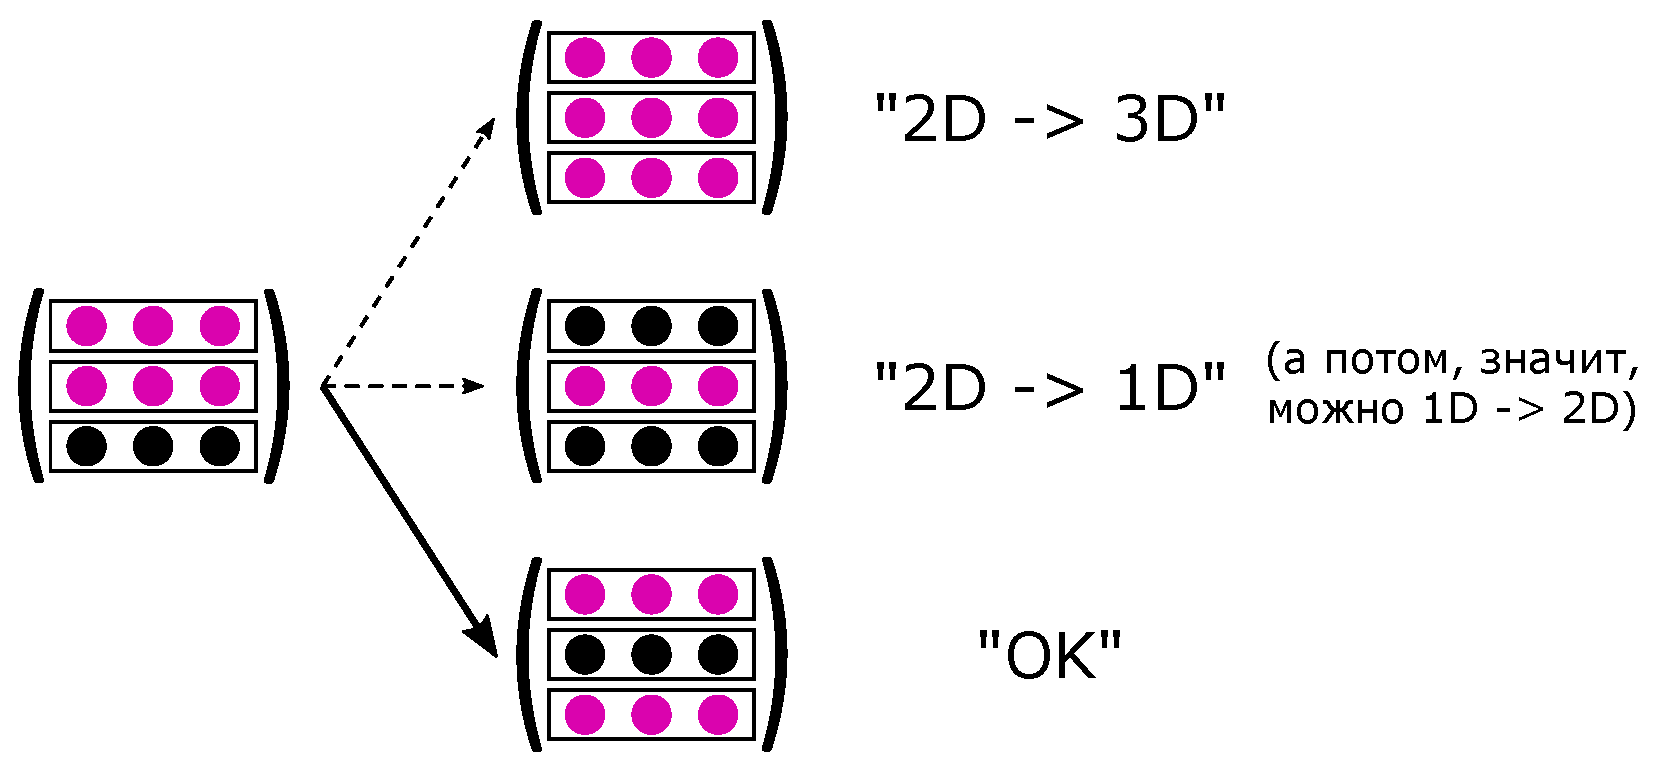
\includegraphics[width=0.8\columnwidth]{elem-rows}
    
      \caption{Максимальное число линейно независимых строк, которые можно выбрать в матрице (строчный ранг), сохраняется при элементарных преобразованиях строк. Если допустить противное, то строчный ранг, получается, может увеличиться или уменьшиться. Если увеличивается, то это словно бы значит, например, что из плоскости (если строчный ранг был равен двум) можно выйти в пространство (если строчный ранг станет равен трём). Если же допустить, что строчный ранг в результате преобразования строк может уменьшиться, то это будет значить, что \emph{обратное} элементарное преобразование увеличивает строчный ранг, чего, по рассмотренному ранее, быть не может.}
      \label{fig:elem-rows}
    \end{figure}
    
    Помимо строк, в любой матрице можно найти и максимальное по количеству подмножество линейно независимых столбцов матрицы (\emph{столбцовый ранг}).
    
    \begin{proposition}
      Элементарное преобразование строк сохраняет столбцовый ранг~(\ref{fig:elem-cols}).
    \end{proposition}
    
    \begin{figure}[h]
      \centering
    
      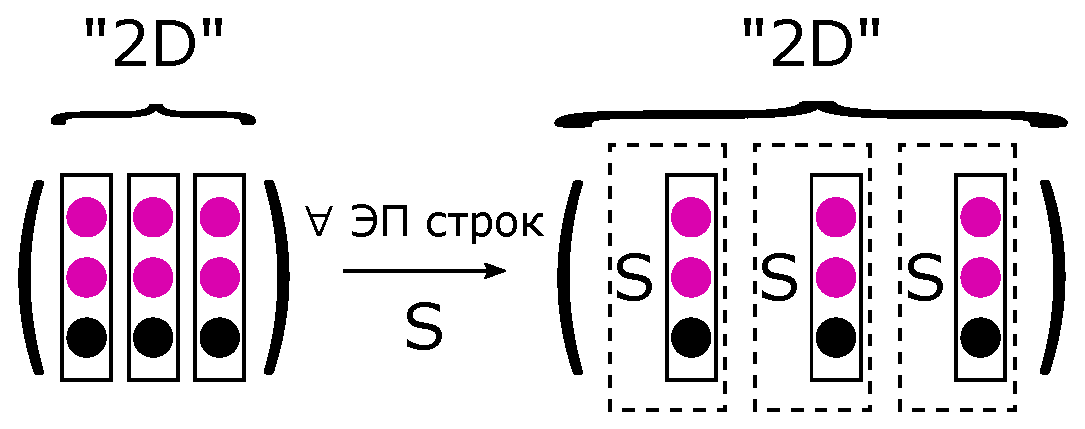
\includegraphics[width=0.8\columnwidth]{elem-cols}
    
      \caption{При элементарных преобразованиях строк сохраняется также и столбцовый ранг. На столбцы матрицы можно смотреть как на координатные столбцы векторов в некотором пространстве, размерность которого равна столбцовому рангу (число координат в столбце может быть больше числа векторов в базисе этого пространства, но это как с плоскостью в трёхмерном пространстве: размерность плоскости равна двум, а векторов в базисе всего векторного пространства три). Под таким углом преобразование строк матрицы, задаваемое матрицей $S$~---~это словно переход к новому базису в описанном подпространстве столбцов (с какой матрицей перехода?). Те столбцы, что были линейно независимы (число которых было равно столбцовому рангу), останутся линейно независимыми; те столбцы, что раскладывались по этой максимальной совокупности линейно независимых (все остальные), с теми же коэффициентами будут раскладываться по тем же столбцам матрицы после преобразования строк.}
      \label{fig:elem-cols}
    \end{figure}
    
    Кроме линейно независимых строк и столбцов в матрице можно найти... максимальную по размеру невырожденную квадратную подматрицу\footnote{Матрица из элементов, стоящих на пересечении выбранных строк и столбцов исходной матрицы (``примерно как'' при зачёркивании строки и столбца при вычислении дополнительного минора).} (``просто'' \emph{ранг}\footnote{Скептически настроенный читатель мог догадаться, что это не общепринятый термин. Можно считать, что такое именование введено только в рамках этого конспекта, чтобы хоть как-то отличать ещё один ранг от введённых ранее строчного и столбцового.}).
    Такая подматрица называется \emph{базисной}.
    
    \begin{example}
      Если исходная матрица квадратная и невырожденная, то она сама и есть эта невырожденная квадратная подматрица максимального размера.
      Если в матрице есть ненулевой элемент, то её ``просто'' ранг точно больше нуля (есть невырожденная подматрица $1 \hm\times 1$).
      Если в матрице разное число строк~$m$ и столбцов~$n$, то ``просто'' ранг не больше~$\min{(m, n)}$.
    \end{example}
    
    Оказывается, что...
    
    \begin{theorem}[О ранге матрицы]
      Строчный, столбцовый и ``просто'' ранги матрицы совпадают.
      Поэтому можно говорить просто о \emph{ранге матрицы}:
      \[
        \Rg\colon \RR^{m\times n} \hm\to \RR
      \]
    \end{theorem}
    
    Почему теорема ``работает''?
    Пусть есть произвольная матрица $A \hm\in \RR^{m \times n}$.
    Попробуем применить к ней метод Гаусса преобразования строк.
    Здесь уже единичной матрицы в итоге может не получиться.
    Может даже оказаться так, что на очередном шаге не получится выбрать ненулевой элемент из столбца.
    Тем не менее, пройдём от первого столбца к последнему (прямой ход) и обратно, ``чистя'' столбцы.
    Матрица, которая получится в результате~(\ref{fig:rang}), называется матрицей, имеющий \emph{упрощённый вид}: некоторые~$r$ её столбцов являются столбцами единичной матрицы, а последние $m \hm- r$ строк нулевые.
    
    Строчный ранг не менялся, в результате же он, очевидно, будет равен~$r$.
    Столбцовый ранг тоже не менялся, и он в упрощённой матрице также будет равен~$r$ (почему?).
    
    Менялся ли ``просто'' ранг?..
    Тоже нет.
    Строки, образующие невырожденную квадратную подматрицу максимального порядка, линейно независимы (почему?).
    Таким образом, строчный ранг матрицы не меньше ``просто'' ранга.
    А значит, увеличиться в процессе преобразований строк ``просто'' ранг не мог.
    Но и уменьшиться он не мог.
    Потому что элементарные преобразования строк обратимы (в другую сторону начинает работать рассуждение с неувеличением).
    
    \begin{figure}[h]
      \centering
    
      \includegraphics[width=0.8\columnwidth]{rang}
    
      \caption{Возможный пример приведения матрицы размера $3 \hm\times 5$ к упрощённому виду с помощью элементарных преобразований строк.}
      \label{fig:rang}
    \end{figure}

  
  \section{Задачи}
  
  
  \subsection{\# 15.45(2)}
  
  Вычислить обратную для матрицы
  \[
    A = \begin{pmatrix}
      2 & -1 & 0\\
      0 & 2 & -1\\
      -1 & -1 & 1
    \end{pmatrix}
  \]
  
  \begin{solution}
    Найдём обратную с помощью метода Гаусса.
    Далее \textcolor{violet}{фиолетовым} цветом будем выделять элемент в столбце, с помощью которого будем занулять другие элементы в том же столбце.
    Те, которые зануляем на данном шаге, будем отмечать \textcolor{red}{красным} цветом.
    Когда столбец ``готов'' (остался один ненулевой~---~фиолетовый), переходим к другому столбцу и снова выбираем ненулевой элемент для ``зачищения столбца'', но \emph{из строчек, откуда ещё не выбирали}.
    Сначала можно занулять все элементы ниже главное диагонали (\emph{прямой ход} метода Гаусса), а потом~---~выше главной диагонали (\emph{обратный ход} метода Гаусса).
    
    \begin{equation*}
    \begin{split}
      &\left(
        \begin{matrix}
          2 & -1 & 0\\
          0 & 2 & -1\\
          -1 & -1 & 1
        \end{matrix}
        \BigMiddleThree
        \begin{matrix}
          1 & 0 & 0\\
          0 & 1 & 0\\
          0 & 0 & 1
        \end{matrix}
        \right)\\
      %
      \widesim{(1) \leftrightarrow (3)}\quad &\left(
        \begin{matrix}
          \textcolor{violet}{\bds{-1}} & -1 & 1\\
          \textcolor{red}{\bds 0} & 2 & -1\\
          \textcolor{red}{\bds 2} & -1 & 0
        \end{matrix}
        \BigMiddleThree
        \begin{matrix}
          0 & 0 & 1\\
          0 & 1 & 0\\
          1 & 0 & 0
        \end{matrix}
        \right)\\
      %
      \widesim{(3) = (3) + 2 \cdot (1)}\quad &\left(
        \begin{matrix}
          -1 & -1 & 1\\
          0 & 2 & -1\\
          0 & -3 & 2
        \end{matrix}
        \BigMiddleThree
        \begin{matrix}
          0 & 0 & 1\\
          0 & 1 & 0\\
          1 & 0 & 2
        \end{matrix}
        \right)\\
      %
      \widesim{(2) = (2) / 2}\quad &\left(
        \begin{matrix}
          -1 & -1 & 1\\
          0 & \textcolor{violet}{\bds 1} & -1/2\\
          0 & \textcolor{red}{\bds{-3}} & 2
        \end{matrix}
        \BigMiddleThree
        \begin{matrix}
          1 & 0 & 0\\
          0 & 1/2 & 0\\
          1 & 0 & 2
        \end{matrix}
        \right)\\
      %
      \widesim{(3) = (3) + 3 \cdot (2)}\quad &\left(
        \begin{matrix}
          -1 & -1 & \textcolor{red}{\bds{1}}\\
          0 & 1 & \textcolor{red}{\bds{-1/2}}\\
          0 & 0 & \textcolor{violet}{\bds{1/2}}
        \end{matrix}
        \BigMiddleThree
        \begin{matrix}
          0 & 0 & 1\\
          0 & 1/2 & 0\\
          1 & 3/2 & 2
        \end{matrix}
        \right)\\
      %
      \widesim{\substack{(1) = (1) - 2 \cdot (3)\\(2) = (2) + (3)}}\quad &\left(
        \begin{matrix}
          -1 & \textcolor{red}{\bds{-1}} & 0\\
          0 & \textcolor{violet}{\bds{1}} & 0\\
          0 & 0 & 1/2
        \end{matrix}
        \BigMiddleThree
        \begin{matrix}
          -2 & -3 & -3\\
          1 & 2 & 2\\
          1 & 3/2 & 2
        \end{matrix}
        \right)\\
      %
      \widesim{\substack{(1) = (1) + (2)\\(3) = 2 \cdot (3)}}\quad &\left(
        \begin{matrix}
          -1 & 0 & 0\\
          0 & 1 & 0\\
          0 & 0 & 1
        \end{matrix}
        \BigMiddleThree
        \begin{matrix}
          -1 & -1 & -1\\
          1 & 2 & 2\\
          2 & 3 & 4
        \end{matrix}
        \right)\\
      %
      \widesim{(1) = -1 \cdot (1)}\quad &\left(
        \begin{matrix}
          1 & 0 & 0\\
          0 & 1 & 0\\
          0 & 0 & 1
        \end{matrix}
        \BigMiddleThree
        \begin{matrix}
          1 & 1 & 1\\
          1 & 2 & 2\\
          2 & 3 & 4
        \end{matrix}
        \right)
    \end{split}
    \end{equation*}
    
    Таким образом,
    \[
      A^{-1} = \begin{pmatrix}
        1 & 1 & 1\\
        1 & 2 & 2\\
        2 & 3 & 4
      \end{pmatrix}
    \]
    
    Можно (стоит) проверить:
    \[
      AA^{-1} = \begin{pmatrix}
        2 & -1 & 0\\
        0 & 2 & -1\\
        -1 & -1 & 1
      \end{pmatrix}
      \cdot \begin{pmatrix}
        1 & 1 & 1\\
        1 & 2 & 2\\
        2 & 3 & 4
      \end{pmatrix}
      = \begin{pmatrix}
        1 & 0 & 0\\
        0 & 1 & 0\\
        0 & 0 & 1
      \end{pmatrix}
    \]
    
    \bigskip
    
    \paragraph{Отступление.}
    
    Найдём интереса ради какую-нибудь $S_i$.
    Например, $S_1$, которая задаёт перестановку строк.
    Правда, перестановка строк~---~не совсем элементарное преобразование.
    Разложим его сначала на элементарные.
    
    Мы хотим задать преобразование перестановки строк (первой и третьей):
    \[
      \begin{pmatrix}
        2 & -1 & 0\\
        0 & 2 & -1\\
        -1 & -1 & 1
      \end{pmatrix}
      \longrightarrow \begin{pmatrix}
        -1 & -1 & 1\\
        0 & 2 & -1\\
        2 & -1 & 0
      \end{pmatrix}
    \]
    
    Это преобразование можно представить как композицию преобразований (над-под каждой стрелочкой обозначено элементарное преобразование и его матрица\footnote{Матрица, которую можно получить, например, из единичной, проведя над её строками аналогичное преобразование.}):
    \begin{equation*}
    \begin{split}
      &\begin{pmatrix}
        2 & -1 & 0\\
        0 & 2 & -1\\
        -1 & -1 & 1
      \end{pmatrix}\\
      \xrightarrow[(3) = (3) + (1)]{\left(\begin{smallmatrix}1 & 0 & 0\\0 & 1 & 0\\1 & 0 & 1\end{smallmatrix}\right)}\quad &\begin{pmatrix}
          2 & -1 & 0\\
          0 & 2 & -1\\
          1 & -2 & 1
        \end{pmatrix}\\
      \xrightarrow[(1) = (1) - (3)]{\left(\begin{smallmatrix}1 & 0 & -1\\0 & 1 & 0\\0 & 0 & 1\end{smallmatrix}\right)}\quad &\begin{pmatrix}
          1 & 1 & -1\\
          0 & 2 & -1\\
          1 & -2 & 1
        \end{pmatrix}\\
      \xrightarrow[(3) = (3) + (1)]{\left(\begin{smallmatrix}1 & 0 & 0\\0 & 1 & 0\\1 & 0 & 1\end{smallmatrix}\right)}\quad &\begin{pmatrix}
          1 & 1 & -1\\
          0 & 2 & -1\\
          2 & -1 & 0
        \end{pmatrix}\\
      \xrightarrow[(1) = -1 \cdot (1)]{\left(\begin{smallmatrix}-1 & 0 & 0\\0 & 1 & 0\\0 & 0 & 1\end{smallmatrix}\right)}\quad &\begin{pmatrix}
          -1 & -1 & 1\\
          0 & 2 & -1\\
          2 & -1 & 0
        \end{pmatrix}
    \end{split}
    \end{equation*}
    
    И в итоге, $S_1$, задающая первую перестановку строк:
    \[
      S_1 = \begin{pmatrix}
          -1 & 0 & 0\\
          0 & 1 & 0\\
          0 & 0 & 1
        \end{pmatrix}
      \cdot \begin{pmatrix}
          1 & 0 & 0\\
          0 & 1 & 0\\
          1 & 0 & 1
        \end{pmatrix}
      \cdot \begin{pmatrix}
          1 & 0 & -1\\
          0 & 1 & 0\\
          0 & 0 & 1
        \end{pmatrix}
      \cdot \begin{pmatrix}
          1 & 0 & 0\\
          0 & 1 & 0\\
          1 & 0 & 1
        \end{pmatrix}
      = \ldots
    \]
  \end{solution}
  
  
  
  \subsection{\# 15.65(3)}
  
  \[
    \begin{pmatrix}
      2 & 1\\
      1 & 1
    \end{pmatrix} X = \begin{pmatrix}
      10\\
      17
    \end{pmatrix}
  \]
  
  \begin{solution}
    Пусть $A \hm\equiv \left(\begin{smallmatrix}
      2 & 1\\
      1 & 1
    \end{smallmatrix}\right)$ и $b \hm\equiv \left(\begin{smallmatrix}
      10\\
      17
    \end{smallmatrix}\right)$.
    
    Какая размерность у матрицы $X$?
    Обозначим размерность матрицы $X$ за $m \hm\times n$ (число строк и число столбцов).
    Тогда имеем:
    \[
      A_{\textcolor{red}{2} \times {\bds 2}} X_{{\bds m} \times \textcolor{cyan}{n}} = b_{\textcolor{red}{2} \times \textcolor{cyan}{1}}
    \]
    
    Поэтому $m \hm= 2$ и $n \hm= 1$.
    
    Также можно заметить, что матрица $A$, которая левый множитель, невырождена.
    
    Как искать $X$?
    
    \bigskip
    
    \paragraph{Способ I: ``По-простому''.}
    
    Пусть $X \hm= \left(\begin{smallmatrix}x \\ y\end{smallmatrix}\right)$.
    Тогда матричное уравнение $AX \hm= b$ равносильно системе из двух скалярных уравнений:
    \[
      \left\{
        \begin{aligned}
          &2x + y = 10\\
          &x + y = 17
        \end{aligned}
      \right.
    \]
    
    Которую можно решить, например, методом Крамера (матрица системы невырождена):
    \[
      \left\{
        \begin{aligned}
          &x = \frac{\left|\begin{smallmatrix}10 & 1 \\ 17 & 1\end{smallmatrix}\right|}{\left|\begin{smallmatrix}2 & 1 \\ 1 & 1\end{smallmatrix}\right|} = \frac{10 - 17}{\det(A)}\\
          &y = \frac{\left|\begin{smallmatrix}2 & 10 \\ 1 & 17\end{smallmatrix}\right|}{\left|\begin{smallmatrix}2 & 1 \\ 1 & 1\end{smallmatrix}\right|} = \frac{2 \cdot 17 - 10}{\det(A)}
        \end{aligned}
      \right.
    \]
    
    
    \medskip
    
    \paragraph{Способ II: ``В контексте темы''.}

    Чтобы найти $X$, можно умножить \emph{слева} обе части уравнения на обратную к матрице-множителю:
    \[
    \underbrace{\begin{pmatrix}
      2 & 1\\
      1 & 1
    \end{pmatrix}^{-1}
    \begin{pmatrix}
      2 & 1\\
      1 & 1
    \end{pmatrix}}_{E} X = \begin{pmatrix}
      2 & 1\\
      1 & 1
    \end{pmatrix}^{-1}
    \begin{pmatrix}
      10\\
      17
    \end{pmatrix}
  \]
  
  В итоге, после нахождения обратной, например, по формуле, получаем:
  \[
    X = \frac{1}{\det(A)} \cdot \begin{pmatrix}
      1 & -1\\
      -1 & 2
    \end{pmatrix}
    \begin{pmatrix}
      10\\
      17
    \end{pmatrix}
    = \frac{1}{\det(A)} \cdot \begin{pmatrix}
      10 - 17\\
      2 \cdot 17 - 10
    \end{pmatrix}
  \]
  \end{solution}
  
  
  \medskip
  
  \emph{Отступление}.
  
  Матрица $A$ в уравнении была невырожденной.
  Посмотрим, что было бы, если бы вместо $A$ в уравнении была другая матрица того же размера $A'$, но вырожденная.
  Например, так:
  \begin{equation}\label{eq:degenerate1}
    \underbrace{\begin{pmatrix}
      1 & 1\\
      1 & 1
    \end{pmatrix}}_{A'} X = \begin{pmatrix}
      10\\
      17
    \end{pmatrix}
  \end{equation}
  
  Очевидно, в таком случае решений нет.
  
  Возьмём другую вырожденную матрицу~$A''$:
  \begin{equation}\label{eq:degenerate2}
    \underbrace{\begin{pmatrix}
      5 & 5\\
      17/2 & 17/2
    \end{pmatrix}}_{A''} X = \begin{pmatrix}
      10\\
      17
    \end{pmatrix}
  \end{equation}
  
  Сводя к системе скалярных уравнений, получаем следующее решение:
  \[
    X = \begin{pmatrix}
      t\\
      2 - t
    \end{pmatrix}
    = \begin{pmatrix}
      0\\
      2
    \end{pmatrix} + \begin{pmatrix}
      1\\
      -1
    \end{pmatrix} t, \quad t \in \RR
  \]
  
  То есть в данном случае решение не просто есть, а их бесконечно много.
  Дело в том, что умножение матрицы справа на столбец $X$ даёт столбец, являющийся линейной комбинацией столбцов матрицы с коэффициентами, записанными в столбец $X$.
  Очевидно, в случае~(\ref{eq:degenerate2}) столбец~$b$ можно разложить по столбцам $A''$, хоть они и линейно зависимы.
  В примере же~(\ref{eq:degenerate1}) столбец~$b$ не может быть представлен как линейная комбинация столбцов~$A'$.
  
  
  
  \subsection{\# 16.19(3)}
  
  \[
    A = \begin{pmatrix}
      1 & 1 & 1\\
      1 & \alpha & \alpha\\
      1 & \alpha^2 & \alpha^2
    \end{pmatrix}
  \]
  \[
    \Rg A = \?
  \]
  
  \begin{solution}
  
    Рассмотрим пару способов решения.
    
    \paragraph{Способ I: ``Наблюдения''.}
    
    В матрице $A$ есть ненулевые элементы, поэтому $\Rg A \hm\geq 1$.
    Второй и третий столбцы матрицы $A$ линейно зависимы, то есть матрица $A$ вырождена, поэтому $\Rg A \hm< 3$.
    Имеет смысл далее рассмотреть систему из первого и, например, второго столбцов матрицы $A$.
    Они линейно зависимы при $\alpha \hm= 1$ (то есть $\Rg A \hm= 1$).
    При всех других $\alpha$ они линейно независимы  (то есть $\Rg A \hm= 2$).
  
    \medskip
    
    \paragraph{Способ II: ``Ещё раз метод Гаусса''.}
    
    Чтобы найти ранг матрицы, можно методом Гаусса привести её к упрощённому виду (то есть ``пытаться'' преобразованиями строк привести матрицу $A \hm\in \RR^{m\times n}$ к единичной: если матрица квадратная и вырожденная или прямоугольная, то некоторые строки в общем случае могут оказаться нулевыми, то есть на очередном шаге метода Гаусса может не получиться найти ненулевой элемент, с помощью которого надо было бы занулять ``лишние'').
    Первым преобразованием можно вычесть первую строку из второй и третьей:
    \[
      \begin{pmatrix}
        1 & 1 & 1\\
        1 & \alpha & \alpha\\
        1 & \alpha^2 & \alpha^2
      \end{pmatrix}
      \longrightarrow
      \begin{pmatrix}
      1 & 1 & 1\\
      0 & \alpha - 1 & \alpha - 1\\
      0 & \alpha^2 - 1 & \alpha^2 - 1
    \end{pmatrix}
    \]
    
    Далее метод Гаусса продолжать сразу нельзя, потому что не понятно, нулевые вторая и третья строки или нет.
    Например, следующим шагом метода Гаусса могла бы быть ``чистка второго столбца'', но для этого во второй или третьей строчке должен быть ненулевой элемент во втором столбце.
    \[
      \alpha = 1 \Rightarrow A = \begin{pmatrix}
        1 & 1 & 1\\
        0 & 0 & 0\\
        0 & 0 & 0
      \end{pmatrix} \Rightarrow \Rg A = 1
    \]
    
    Пусть $\alpha \hm{\not=} 1$.
    Тогда вторая строчка ненулевая, и можно её (и третью строчку тоже) поделить на $\alpha - 1$:
    \[
      \begin{pmatrix}
        1 & 1 & 1\\
        0 & \alpha - 1 & \alpha - 1\\
        0 & \alpha^2 - 1 & \alpha^2 - 1
      \end{pmatrix}
      \longrightarrow
      \begin{pmatrix}
        1 & 1 & 1\\
        0 & 1 & 1\\
        0 & \alpha + 1 & \alpha + 1
      \end{pmatrix}
    \]
    
    Вне зависимости от того, нулевая третья строчка или нет, её можно занулить, вычтя с нужным коэффициентом вторую.
    То есть
    \[
      \begin{pmatrix}
        1 & 1 & 1\\
        0 & 1 & 1\\
        0 & \alpha + 1 & \alpha + 1
      \end{pmatrix}
      \longrightarrow
      \begin{pmatrix}
        1 & 1 & 1\\
        0 & 1 & 1\\
        0 & 0 & 0
      \end{pmatrix}
      \longrightarrow
      \begin{pmatrix}
        1 & 0 & 0\\
        0 & 1 & 1\\
        0 & 0 & 0
      \end{pmatrix}
    \]
    
    Привели матрицу $A$ к упрощённому виду (в первых строках можно найти подматрицу единичной матрицы, а остальные строки~---~нулевые).
    Ранг у упрощённой матрицы равен двум.
    Поэтому и $\Rg A \hm= 2$ (при $\alpha \hm{\not=} 1$).
  \end{solution}
\end{document}
